%% IEEE-format revision of the FDP-on-NVMeVirt paper.
%% Builds with: pdflatex paper_ieee && bibtex paper_ieee && pdflatex x2
%% The original USENIX paper (paper.tex / paper.pdf) is left untouched.
\documentclass[conference,10pt]{IEEEtran}

\usepackage{graphicx}
\usepackage{booktabs}
\usepackage{amsmath}
\usepackage{amssymb}
\usepackage{xcolor}
\usepackage{tikz}
\usetikzlibrary{positioning,fit,backgrounds,arrows.meta}
\usepackage{ifthen}
\usepackage[hidelinks]{hyperref}
\usepackage{url}

\IEEEoverridecommandlockouts
\emergencystretch=3em  % absorb rare small overfull lines without bad spacing

\definecolor{hotc}{HTML}{C0392B}
\definecolor{coldc}{HTML}{2471A3}

\begin{document}

\title{Bringing Flexible Data Placement to NVMeVirt:\\
A Software-Defined FDP SSD for Storage Research}

\author{%
\IEEEauthorblockN{Sinu Lee}
\IEEEauthorblockA{Dept.\ of Computer Science\\and Engineering\\Seoul National University}
\and
\IEEEauthorblockN{Bosung An}
\IEEEauthorblockA{Dept.\ of Electrical and\\Computer Engineering\\Seoul National University}
\and
\IEEEauthorblockN{Jonghyeon Park}
\IEEEauthorblockA{Dept.\ of Computer Science\\and Engineering\\Seoul National University}}

\maketitle

\begin{abstract}
Flexible Data Placement (FDP) is a recent NVMe feature that lets the host hint
\emph{where} data is placed on a flash device so that data of similar lifetime
shares the same physically reclaimed region, reducing garbage-collection (GC)
write amplification without abandoning the conventional block interface.
Studying FDP, however, requires FDP-capable hardware, which remains scarce, and
no open emulator exposes the feature to an unmodified host stack. We extend
NVMeVirt, a software-defined virtual NVMe device implemented as a Linux kernel
module, into a functional FDP SSD. It advertises the FDP capability, serves the
FDP log pages and features, performs host-directed placement into
per-Reclaim-Unit-Handle (RUH) reclaim units, and reports FDP events. The emulated
device is driven end to end by the unmodified in-kernel NVMe driver and
\texttt{nvme-cli}. Using a synthetic
hot/cold workload that models two data lifetimes, we show that FDP placement
reduces write amplification by up to 61\% (a $2.5\times$ flash-endurance gain)
relative to an \emph{identical} device with placement disabled, and we
characterize how the benefit depends on over-provisioning and workload skew. We
then reproduce the effect on a RocksDB-like log-structured-merge workload, where
mapping LSM levels to separate reclaim units cuts write amplification by 34\%
and reveals how many reclaim units a deployment actually needs.
The extension and all evaluation artifacts are publicly available.
\end{abstract}

\begin{IEEEkeywords}
NVMe, Flexible Data Placement, flash storage, garbage collection, write
amplification, SSD emulation.
\end{IEEEkeywords}

%===============================================================================
\section{Introduction}
%===============================================================================
NAND flash cannot be overwritten in place: a page must be erased before reuse,
and erases act on large blocks. Flash devices therefore write out-of-place and
reclaim stale space with a garbage collector (GC) that must relocate any
still-valid pages out of a victim block before erasing it. This relocation is
pure overhead, since it spends flash program and erase cycles that do no useful
host work. We capture it with the \emph{write amplification factor} (WAF), the
ratio of bytes written to the media to bytes written by the host. A high WAF
degrades throughput, tail latency, and endurance~\cite{arpachiDusseau18:osbook}.

A decades-long line of work observes that WAF collapses when each erase block
holds data of a single \emph{lifetime}: if everything in a block dies at about
the same time, the block is reclaimed with little or no
copying~\cite{lifetime:hotcold,lfs:tocs92}. The obstacle is information: the
device does not know application lifetimes, only the host does. NVMe
\emph{Flexible Data Placement} (FDP)~\cite{fdp:tp4146} closes this gap. The host
attaches a \emph{placement} hint to each write, and the device co-locates writes
that share a hint into the same \emph{Reclaim Unit} (RU). Crucially, placement
is only a \emph{hint}: a write with no directive uses a default RU, so legacy
software runs unchanged. This advisory, block-interface-preserving design is the
key distinction from Zoned Namespaces (ZNS)~\cite{zns:atc21}, which replaces the
block interface with append-only zones, and a standardization of multi-streamed
SSDs~\cite{multistream:hotstorage14}.

\textbf{The problem.} Despite strong industry momentum, FDP is hard to study in
academia: FDP-capable drives are scarce, and existing open SSD emulators do not
implement it. FEMU~\cite{femu:fast18} and MQSim~\cite{mqsim:fast18} model flash
timing but expose no FDP interface, and neither presents the feature to a real,
unmodified NVMe stack. Researchers therefore cannot answer even basic questions
(\emph{when}, and by \emph{how much}, does FDP help?) on commodity machines.

\textbf{Our approach.} We build on NVMeVirt~\cite{nvmevirt:fast23}, which
fabricates a virtual NVMe controller at the PCIe layer inside a Linux kernel
module, so the device is driven by the \emph{unmodified} in-kernel NVMe driver
and standard tools. NVMeVirt ships conventional-SSD, ZNS, and key-value targets
but not FDP. We add a complete FDP device model and use it to quantify FDP's
benefit on commodity hardware with no special drivers.

\textbf{Contributions.}
\begin{itemize}
\item A functional NVMe FDP device model for NVMeVirt: Identify-level capability
advertisement, the four FDP log pages (configurations, RUH usage, statistics,
events) and both FDP features, host-directed placement into per-RUH reclaim
units, invalid-placement handling, and FDP event reporting
(\S\ref{sec:design}), validated against \texttt{nvme-cli}.
\item An evaluation methodology and a two-phase synthetic lifetime workload that
drive the emulated device entirely through the standard NVMe passthrough
interface (\S\ref{sec:method}).
\item A characterization showing up to 61\% WAF reduction ($2.5\times$
endurance) from placement, together with a sweep that explains how the benefit
depends on over-provisioning and workload skew, and therefore \emph{when} FDP is
worthwhile; and a confirmation of the effect on a RocksDB-like LSM workload that
also shows how many reclaim units a deployment needs (\S\ref{sec:eval}).
\end{itemize}

%===============================================================================
\section{Background and Motivation}
\label{sec:bg}
%===============================================================================

\subsection{Garbage collection and write amplification}
A flash translation layer (FTL) maps logical pages to physical pages and writes
updates to a clean ``write frontier.'' When clean space runs low, GC selects a
victim block (typically lowest valid-page count), copies its valid pages to the
frontier, and erases it. If a victim mixes soon-to-die and long-lived data, the
long-lived pages are copied \emph{repeatedly} across GC cycles, inflating WAF.
Over-provisioning (OP), the physical capacity beyond the exported logical
capacity, gives GC more slack and lowers WAF, at the cost of usable space. The
governing tension is therefore between how full the device is (set by OP) and how
mixed each block is (set by lifetime separation).

\subsection{Why placement helps: the mixing problem}
Figure~\ref{fig:concept} illustrates the effect that FDP exploits. Under a
skewed hot/cold workload, a placement-agnostic device interleaves hot and cold
logical addresses into the same physical lines (left). When the hot data is
rewritten, it leaves holes scattered across \emph{many} lines, each still
pinning a few cold survivors; GC must copy those survivors before it can erase,
and it pays this cost again every time the line refills. With placement (right),
hot and cold data occupy separate lines from the start; a hot line becomes
\emph{entirely} invalid and is reclaimed with \emph{zero} copying, while the cold
lines are rarely touched. The GC algorithm itself does not change. The host has
simply stopped mixing lifetimes within a line.

\begin{figure}[t]
\centering
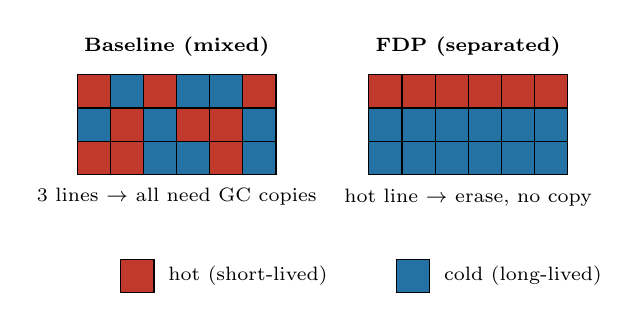
\begin{tikzpicture}[every node/.style={font=\scriptsize}]
  \def\cs{0.42}
  % ---- Baseline (left): fixed mixed pattern per row ----
  \node[font=\scriptsize\bfseries] at (3*\cs,1.62) {Baseline (mixed)};
  \foreach[count=\ri] \row in {{h,c,h,c,c,h},{c,h,c,h,h,c},{h,h,c,c,h,c}} {
    \pgfmathsetmacro\yy{(3-\ri)*\cs}
    \foreach[count=\ci] \cell in \row {
      \pgfmathsetmacro\xx{(\ci-1)*\cs}
      \ifthenelse{\equal{\cell}{h}}
        {\fill[hotc] (\xx,\yy) rectangle ++(\cs,\cs);}
        {\fill[coldc] (\xx,\yy) rectangle ++(\cs,\cs);}
      \draw (\xx,\yy) rectangle ++(\cs,\cs);
    }
  }
  \node at (3*\cs,-0.28) {3 lines $\to$ all need GC copies};
  % ---- FDP (right) ----
  \begin{scope}[xshift=3.7cm]
  \node[font=\scriptsize\bfseries] at (3*\cs,1.62) {FDP (separated)};
  \foreach[count=\ri] \row in {{h,h,h,h,h,h},{c,c,c,c,c,c},{c,c,c,c,c,c}} {
    \pgfmathsetmacro\yy{(3-\ri)*\cs}
    \foreach[count=\ci] \cell in \row {
      \pgfmathsetmacro\xx{(\ci-1)*\cs}
      \ifthenelse{\equal{\cell}{h}}
        {\fill[hotc] (\xx,\yy) rectangle ++(\cs,\cs);}
        {\fill[coldc] (\xx,\yy) rectangle ++(\cs,\cs);}
      \draw (\xx,\yy) rectangle ++(\cs,\cs);
    }
  }
  \node at (3*\cs,-0.30) {hot line $\to$ erase, no copy};
  \end{scope}
  % legend (single row, well below the panels; wide gap so the hot label
  % cannot run into the cold swatch)
  \fill[hotc] (0.55,-1.5) rectangle ++(\cs,\cs); \draw (0.55,-1.5) rectangle ++(\cs,\cs);
  \node[anchor=west] at (0.55+\cs+0.06,-1.5+\cs/2) {hot (short-lived)};
  \fill[coldc] (4.05,-1.5) rectangle ++(\cs,\cs); \draw (4.05,-1.5) rectangle ++(\cs,\cs);
  \node[anchor=west] at (4.05+\cs+0.06,-1.5+\cs/2) {cold (long-lived)};
\end{tikzpicture}
\caption{Lifetime mixing. Without placement, hot rewrites strand cold survivors
in many lines, forcing repeated GC copies; FDP places lifetimes in separate
lines, so a hot line is reclaimed with no copying.}
\label{fig:concept}
\end{figure}

\subsection{NVMe Flexible Data Placement}
FDP~\cite{fdp:tp4146} adds host-directed placement to the NVM command set,
scoped to an \emph{endurance group}. The host references a Reclaim Unit Handle
(RUH) through a placement identifier carried in the write command's directive
fields; the device steers all writes sharing an RUH into the same RU, the
granularity at which media is reclaimed. FDP is exposed through Identify fields,
four log pages (configurations, RUH usage, statistics, events), and two features
(FDP, FDP-events). A write without a placement directive uses a default RUH, so
unmodified software keeps working. This property is what sets FDP apart from ZNS,
and it makes FDP an attractive incremental path to lifetime-aware placement.

%===============================================================================
\section{Related Work}
\label{sec:related}
%===============================================================================
\textbf{Lifetime-aware placement.} Clustering data by update frequency to lower
cleaning cost originates in log-structured file systems~\cite{lfs:tocs92} and
early flash cleaning policies~\cite{lifetime:hotcold}. Multi-streamed
SSDs~\cite{multistream:hotstorage14} first exposed a host placement hint at the
device interface; subsequent systems automated stream assignment from access
patterns (AutoStream~\cite{autostream:systor17}), file-system hints
(FStream~\cite{fstream:fast18}), or program contexts
(PCStream~\cite{pcstream:fast19}). FDP~\cite{fdp:tp4146} generalizes streams into
a standardized, endurance-group-scoped mechanism with an explicit reclaim-unit
model and statistics/event reporting. Open-Channel SSDs~\cite{lightnvm:fast17}
and ZNS~\cite{zns:atc21} push placement control further by exposing physical
geometry or append-only zones, at the cost of host complexity and a broken block
interface; FDP keeps the block interface and treats placement as advisory.
Lifetime separation also appears one level up the stack, for example in the
key/value separation of WiscKey~\cite{wisckey:fast16} and in the flash-friendly
design of F2FS~\cite{f2fs:fast15}; these are complementary hint \emph{sources}
for an FDP device. Table~\ref{tab:taxonomy} situates these mechanisms.

\begin{table}[t]
\centering
\caption{Host-directed placement interfaces.}
\label{tab:taxonomy}
\footnotesize
\begin{tabular}{lccc}
\toprule
Mechanism & Block iface & Placement & Legacy host \\
\midrule
Conventional SSD            & yes & none (device) & yes \\
Multi-stream~\cite{multistream:hotstorage14} & yes & stream hint & yes \\
Open-Channel~\cite{lightnvm:fast17} & no  & full geometry & no \\
ZNS~\cite{zns:atc21}        & no  & append zones  & no \\
\textbf{FDP}~\cite{fdp:tp4146} & \textbf{yes} & \textbf{RUH hint} & \textbf{yes} \\
\bottomrule
\end{tabular}
\end{table}

\textbf{SSD emulation.} FEMU~\cite{femu:fast18} is a QEMU-based NVMe flash
emulator and MQSim~\cite{mqsim:fast18} a detailed discrete-event device
simulator; both model timing but expose no FDP interface, and a simulator is not
driven by the real OS stack. NVMeVirt~\cite{nvmevirt:fast23} instead emulates at
the PCIe layer inside the kernel, so the unmodified NVMe driver binds to it and
userspace sees an ordinary \texttt{/dev/nvme*}. We extend NVMeVirt precisely for
this property: an FDP model that real tools (\texttt{nvme-cli}, passthrough
ioctls) exercise without modification. To our knowledge this is the first open
FDP device model usable by an unmodified host stack.

%===============================================================================
\section{NVMeVirt FDP Extension}
\label{sec:design}
%===============================================================================
NVMeVirt presents a virtual NVMe controller at the PCIe layer: a dispatcher
thread polls the controller's doorbell registers, decodes each submission-queue
entry, and routes it either to the admin handler or, for I/O, through a
per-namespace handler (\texttt{ns->proc\_io\_cmd}) to a pluggable FTL. We add FDP
as a new namespace target and reuse this structure wholesale
(Fig.~\ref{fig:arch}). Our FTL is forked from NVMeVirt's conventional-SSD FTL,
which already supplies everything FDP's data path needs: a write frontier,
super-block \emph{lines} as the reclaim granularity, line-based garbage
collection, and a NAND timing model.

\begin{figure}[t]
\centering
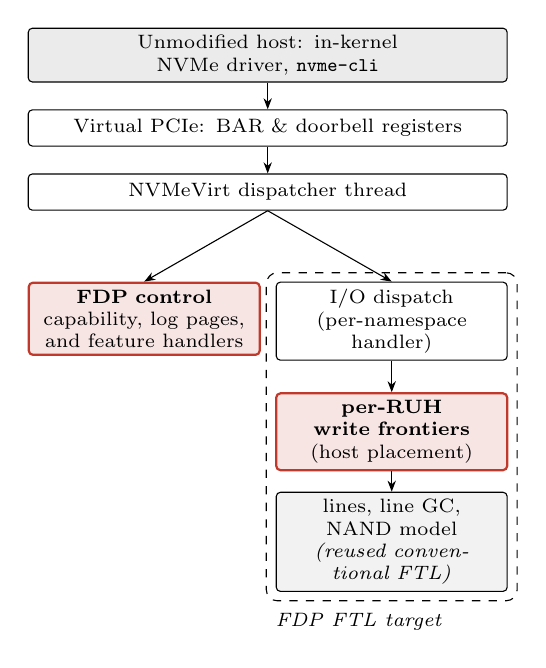
\begin{tikzpicture}[font=\scriptsize, >={Stealth[length=4pt]},
  box/.style={draw, rounded corners=1.5pt, align=center, inner sep=2.6pt,
              minimum height=4.6mm, text width=5.9cm},
  sm/.style={draw, rounded corners=1.5pt, align=center, inner sep=2.6pt,
             minimum height=4.6mm, text width=2.75cm},
  new/.style={fill=hotc!13, draw=hotc, thick},
  reuse/.style={fill=black!5},
  node distance=3.4mm]
  \node[box, fill=black!8] (host) {Unmodified host: in-kernel NVMe driver, \texttt{nvme-cli}};
  \node[box, below=of host] (pcie) {Virtual PCIe: BAR \& doorbell registers};
  \node[box, below=of pcie] (disp) {NVMeVirt dispatcher thread};
  \node[sm, new, below=9mm of disp.south west, anchor=north west] (admin)
        {\textbf{FDP control}\\capability, log pages,\\and feature handlers};
  \node[sm, below=9mm of disp.south east, anchor=north east] (io)
        {I/O dispatch\\(per-namespace handler)};
  \node[sm, new, below=4mm of io] (wp)
        {\textbf{per-RUH write frontiers}\\(host placement)};
  \node[sm, reuse, below=2.6mm of wp] (nand)
        {lines, line GC, NAND model\\\emph{(reused conventional FTL)}};
  \draw[->] (host)--(pcie);
  \draw[->] (pcie)--(disp);
  \draw[->] (disp.south) -- (admin.north);
  \draw[->] (disp.south) -- (io.north);
  \draw[->] (io)--(wp);
  \draw[->] (wp)--(nand);
  \begin{scope}[on background layer]
    \node[draw, dashed, rounded corners, fit=(io)(wp)(nand), inner sep=3.2pt] (ftl) {};
  \end{scope}
  \node[anchor=north west, font=\scriptsize\itshape] at ([yshift=-0.3mm]ftl.south west) {FDP FTL target};
\end{tikzpicture}
\caption{The FDP target reuses NVMeVirt's PCIe front end, dispatcher, and the
conventional FTL's lines, garbage collection, and timing model. The shaded boxes
are the only additions: the FDP control surface and the per-RUH write frontiers.}
\label{fig:arch}
\end{figure}

The single substantive change to the data path is to keep \emph{one write
frontier per reclaim unit handle} (eight in our configuration) rather than one
global frontier. Each handle owns its own open line, so every reclaim unit it
opens starts out separate from the others. We therefore expose all handles as the
\emph{initially isolated} reclaim-unit-handle type, the FDP mode in which a newly
referenced reclaim unit does not share media with any other handle, which is
exactly the behavior our one-line-per-handle design provides. On each write we
read the command's placement directive: a placement-tagged write is steered to
the addressed RUH's frontier, while an untagged write falls back to a default
RUH. Writes that carry different placement identifiers therefore land in
different physical lines, so it is the host, not the device, that decides which
data shares a reclaim unit. We leave garbage
collection untouched and placement-agnostic, so it relocates survivors to a
shared frontier just as before. This choice is deliberate, because it ensures
that any benefit we measure comes from placement alone and not from a smarter
cleaning policy.

Around this data path we add the FDP control surface a standards-compliant host
expects, so an unmodified Linux stack and \texttt{nvme-cli} drive the device
without changes. The controller and namespace advertise FDP in Identify; the
four FDP log pages report the configuration, per-RUH usage, the host/media/erase
byte counters, and a ring of recent events; and the two FDP features expose the
enable state and a settable event mask. Because host writes increment both the
host- and media-written counters while GC copies increment only the media
counter, the statistics log yields the write-amplification factor
$\mathrm{WAF}=\mathrm{MBMW}/\mathrm{HBMW}$ directly, and this is the quantity our
evaluation reads back. We confirmed with \texttt{nvme-cli} that the capability
bits, all of the log pages, and both features decode correctly, that a placement
directive marks the addressed RUH as host-specified, and that an out-of-range
identifier is rejected and recorded as an FDP event.

%===============================================================================
\section{Methodology}
\label{sec:method}
%===============================================================================
We run NVMeVirt with the FDP target inside a lightweight VM that boots the host
kernel, so the build is exercised by the real Linux NVMe stack and
\texttt{nvme-cli}. Table~\ref{tab:params} lists the configuration.

\begin{table}[t]
\centering
\caption{Experimental configuration.}
\label{tab:params}
\footnotesize
\begin{tabular}{ll}
\toprule
Parameter & Value \\
\midrule
Emulator / target      & NVMeVirt $+$ FDP, \texttt{SAMSUNG\_FDP} \\
Host \& guest kernel   & Linux 6.12 (virtme-ng) \\
Device capacity        & 64\,MiB, 4 FTL partitions \\
Reclaim unit handles   & 8 (1 reclaim group, 1 endurance grp) \\
Intrinsic over-prov.   & $\approx$7\% \\
Write size             & 32\,KiB via NVMe passthrough \\
Hot region / hot writes& 20\% of LBAs / 90\% of writes (default) \\
Metric                 & $\mathrm{WAF}=\mathrm{MBMW}/\mathrm{HBMW}$ (statistics log) \\
\bottomrule
\end{tabular}
\end{table}

\textbf{Metric.} WAF is read from the FDP Statistics log. It depends only on FTL
logic and the workload, not on wall-clock timing, so it is valid under CPU-only
emulation; it also maps directly to endurance,
$\text{endurance gain}=\mathrm{WAF}_{\text{base}}/\mathrm{WAF}_{\text{FDP}}$.

\textbf{Workload.} A two-phase generator models two lifetime classes. First a
\emph{random-order fill} writes the working set once; random order is essential
so that, \emph{without} placement, hot and cold addresses interleave into the
same lines (Fig.~\ref{fig:concept}). Then a \emph{churn} phase rewrites the hot
set repeatedly. We compare two configurations on the \emph{same} device and
workload: a \textbf{baseline} issuing no placement directive (all data to the
default RUH), and \textbf{FDP} placing hot data in one RUH and cold data in
another. WAF is measured as a \emph{delta over the churn phase only} (statistics
snapshotted after the fill), so the near-unit WAF of the fill does not dilute the
steady-state number; each measurement uses a freshly loaded device with reset
counters. The design isolates a single variable, namely whether writes carry a
placement directive, so any difference we see is attributable to placement alone.

\textbf{Device sizing.} We deliberately use a small device so GC reaches steady
state at a tractable write volume under emulation; the block geometry is scaled
so that physical capacity tracks the requested logical capacity (the intended
$\approx$7\% OP) rather than leaving so much implicit over-provisioning that GC
never runs. Trends are geometry-independent; absolute WAF scales with OP and
working set, which is exactly what the sweeps in \S\ref{sec:eval} characterize.

%===============================================================================
\section{Evaluation}
\label{sec:eval}
%===============================================================================
We answer four questions: (1) how much does placement reduce write
amplification at a representative operating point; (2) how does the benefit vary
with over-provisioning; (3) how does it vary with workload separability; and
(4) does the effect carry over to a realistic, multi-stream access pattern.
Across all of them the result is one-directional: FDP \emph{reduces} write
amplification in every configuration we measured and never increases it,
by 34--61\% where garbage collection is active (a $1.5$--$2.5\times$ endurance
gain). The size of the win grows with workload separability and garbage-collection
pressure and shrinks toward zero when either is absent. A built-in control
pins the cause to placement rather than any artifact: running FDP with a single
reclaim unit (so no lifetime can be separated) reproduces the baseline WAF
exactly (\S\ref{sec:lsm}).

\subsection{Write-amplification reduction}
At the operating point (90\% working set, 90\% of writes into the 20\% hot
region), both configurations issue identical host writes, but the baseline pushes
$6.0\times$ that volume to the media against $3.2\times$ for FDP, a 47\% reduction
(Table~\ref{tab:headline}). The bytes-erased counter (MBE) points to the cause:
FDP erases 49\% fewer bytes, which means GC runs far less often because hot lines
are reclaimed without copying. The baseline pays its cost copying the cold pages
that are stranded in hot-dominated lines, which is exactly the mixing that FDP
avoids.

\begin{table}[t]
\centering
\caption{Operating point: identical host writes, 47\% less media traffic and
49\% fewer erased bytes under FDP.}
\label{tab:headline}
\footnotesize
\begin{tabular}{lrrrr}
\toprule
 & $\Delta$HBMW & $\Delta$MBMW & MBE & WAF \\
\midrule
Baseline & 20.0\,MiB & 120.4\,MiB & 118.0\,MiB & 6.02 \\
FDP      & 20.0\,MiB & 63.4\,MiB  & 60.5\,MiB  & 3.17 \\
\bottomrule
\end{tabular}
\end{table}

\subsection{Effect of over-provisioning}
Figure~\ref{fig:op} sweeps the working-set size (hence free space/OP) at fixed
skew. The FDP benefit is largest at \emph{moderate} OP: with abundant free space
(75\% working set, $\sim$33\% OP) GC seldom runs and neither configuration
amplifies, while under extreme pressure (96\%, $\sim$4\% OP) the device is nearly
full and even FDP must copy to make room. In between, FDP roughly halves WAF; at
a 92\% working set, for instance, it drops from $10.1\times$ to $4.6\times$, a
55\% reduction. This non-monotonic shape matches the intuition that placement
helps only when GC is both active and avoidable, and it tells a practitioner the
regime in which FDP pays off.

\begin{figure}[t]
\centering
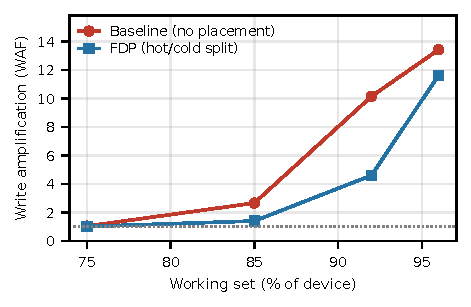
\includegraphics[width=0.92\columnwidth]{fig_op.pdf}
\caption{WAF vs.\ over-provisioning (working-set size, fixed skew). FDP's
advantage peaks at moderate OP and shrinks at both extremes.}
\label{fig:op}
\end{figure}

\subsection{Effect of workload skew}
Figure~\ref{fig:skew} varies the fraction of writes hitting the hot region at
fixed working set. The baseline WAF stays essentially flat at about 5.5, because
mixing lifetimes hurts it regardless of skew, while FDP's WAF falls steadily as
the workload becomes more separable, from $3.95\times$ at 70\% to $2.17\times$ at
95\%. The reduction grows from 31\% to 61\%, a $1.5\times$ to $2.5\times$
endurance gain (Fig.~\ref{fig:endurance}). In other words, the cleaner the
lifetime separation the host can express, the more FDP delivers, which is the
core FDP value proposition shown directly.

\begin{figure}[t]
\centering
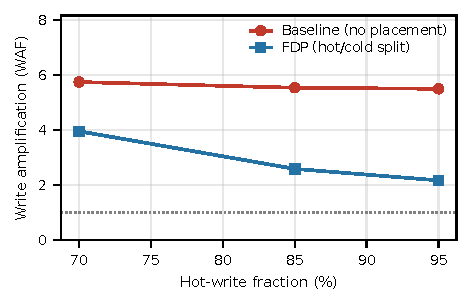
\includegraphics[width=0.92\columnwidth]{fig_skew.pdf}
\caption{WAF vs.\ workload skew (hot-write fraction, fixed working set). Baseline
is flat; FDP improves monotonically as lifetimes separate.}
\label{fig:skew}
\end{figure}

\begin{figure}[t]
\centering
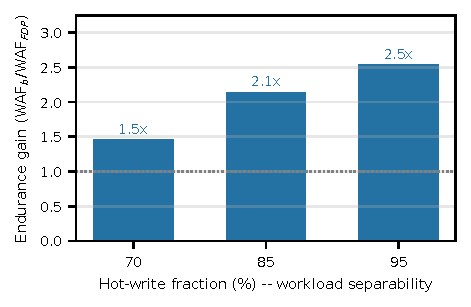
\includegraphics[width=0.92\columnwidth]{fig_endurance.pdf}
\caption{Endurance gain ($\mathrm{WAF}_{\text{base}}/\mathrm{WAF}_{\text{FDP}}$)
across the skew sweep, reaching $2.5\times$ at the most separable point.}
\label{fig:endurance}
\end{figure}

\subsection{Variance}
Table~\ref{tab:var} repeats the operating point under two random seeds, at the
lighter per-point churn used throughout the sweeps. The headline of
Table~\ref{tab:headline} uses a deeper churn that drives the device closer to
steady state, which is why its absolute WAF sits a little higher; the
baseline-to-FDP ratio, which is what we report, is consistent across both. Across
seeds the baseline and FDP WAF each move by only about $\pm2\%$, well below the
$2$ to $3\times$ baseline-to-FDP gaps, so single-seed points are representative.
The consolidated sweep data appear in Table~\ref{tab:sweep}.

\begin{table}[t]
\centering
\caption{Seed variance at the operating point ($\pm2\%$).}
\label{tab:var}
\footnotesize
\begin{tabular}{lrr}
\toprule
Seed & Baseline WAF & FDP WAF \\
\midrule
1 & 5.41 & 2.57 \\
2 & 5.66 & 2.38 \\
\bottomrule
\end{tabular}
\end{table}

\begin{table}[t]
\centering
\caption{Consolidated sweep results. OP sweep at fixed 90\% skew; skew sweep at
fixed 90\% working set.}
\label{tab:sweep}
\footnotesize
\begin{tabular}{llrrrr}
\toprule
Sweep & Point & Base & FDP & Reduc. & Endur. \\
\midrule
OP   & 75\% WS ($\sim$33\% OP) & 1.03  & 1.01  & 2\%  & 1.0$\times$ \\
OP   & 85\% WS ($\sim$18\% OP) & 2.66  & 1.40  & 47\% & 1.9$\times$ \\
OP   & 92\% WS ($\sim$9\% OP)  & 10.15 & 4.60  & 55\% & 2.2$\times$ \\
OP   & 96\% WS ($\sim$4\% OP)  & 13.41 & 11.62 & 13\% & 1.2$\times$ \\
\midrule
Skew & 70\% hot writes & 5.74 & 3.95 & 31\% & 1.5$\times$ \\
Skew & 85\% hot writes & 5.54 & 2.59 & 53\% & 2.1$\times$ \\
Skew & 95\% hot writes & 5.50 & 2.17 & 61\% & 2.5$\times$ \\
\bottomrule
\end{tabular}
\end{table}

\subsection{A RocksDB-like LSM workload}
\label{sec:lsm}
The sweeps above use a controlled two-class workload. To check whether the same
effect appears on a realistic access pattern, and to use more than two reclaim
units, we drive the device with an I/O stream modeled on a log-structured-merge
(LSM) tree, the structure behind RocksDB and the canonical FDP use case. Under
leveled compaction, level $i$ holds on the order of $T^i$ times as much data as
the top level (fanout $T$), and data in a level is rewritten about once per
level-fill, which happens roughly $T$ times more often than in the level below.
Data lifetime therefore tracks the level: the top level is small and churns
quickly, the bottom level is large and is rarely rewritten, and adjacent levels
differ in update rate by about $T$. The \emph{level} is thus a natural lifetime
class, and ``one level per reclaim unit'' is exactly the mapping that
RocksDB-on-FDP deployments use. We generate this stream directly from the level
geometry (default $T=4$, four levels) rather than running RocksDB, so the
experiment stays self-contained while its hot/cold structure comes from the data
structure rather than an arbitrary knob.

Figure~\ref{fig:lsm} sweeps how many reclaim unit handles hold the levels, from
one (all data in a single reclaim unit, equivalent to the baseline) up to one
per level. With a single handle, FDP reproduces the baseline WAF of $6.6$
exactly---a built-in sanity check, since one reclaim unit cannot separate
anything. WAF then falls monotonically as more levels get their own handle,
reaching $4.3$ with one handle per level: a 34\% reduction, or a $1.5\times$
endurance gain. The curve has a clear knee---isolating the fast-churning top
level first yields the largest single improvement and each additional handle
helps less---which is direct guidance on how many reclaim units a deployment
actually needs. The reduction is smaller than the two-class operating point
(47\%) because leveled compaction spreads churn across all levels rather than
concentrating it in a tiny hot region; even so, it confirms the placement
effect on a workload whose lifetimes arise from a real data structure rather
than a synthetic hot/cold knob.

\begin{figure}[t]
\centering
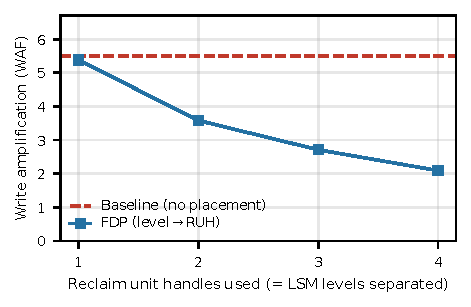
\includegraphics[width=0.92\columnwidth]{fig_lsm_ruh.pdf}
\caption{RocksDB-like LSM workload: WAF vs.\ the number of reclaim unit handles
used to separate LSM levels. One handle reproduces the baseline; the first split
gives the largest single gain, and one handle per level cuts WAF by 34\%.}
\label{fig:lsm}
\end{figure}

\begin{table}[t]
\centering
\caption{RocksDB-like LSM workload ($T{=}4$, 4 levels): WAF vs.\ reclaim unit
handles used. $N{=}1$ (single reclaim unit) reproduces the baseline.}
\label{tab:lsm}
\footnotesize
\begin{tabular}{rrrrr}
\toprule
RUHs ($N$) & Baseline & FDP & Reduc. & Endur. \\
\midrule
1 & 6.58 & 6.58 & 0\%  & 1.0$\times$ \\
2 & 6.58 & 5.66 & 14\% & 1.2$\times$ \\
3 & 6.58 & 4.96 & 25\% & 1.3$\times$ \\
4 & 6.58 & 4.32 & 34\% & 1.5$\times$ \\
\bottomrule
\end{tabular}
\end{table}

\subsection{Discussion and limitations}
The results isolate the placement effect: baseline and FDP differ only in
whether writes carry a directive, on the same device and FTL. Two limitations
follow from the setup. First, we report WAF and endurance rather than throughput
or latency, because NVMeVirt's timing model is not faithful under pure CPU
emulation, so performance numbers would require a bare-metal run. This is a
natural next step now that the functional model exists. Second, our workloads are
generated rather than captured: the two-class sweeps use the standard hot/cold
lifetime abstraction, and the LSM experiment is driven by a model of leveled
compaction rather than a live RocksDB instance. Replaying a captured trace from a
running application would further strengthen external validity, and our
standard-interface design makes that straightforward. Finally, GC currently
reclaims to a shared frontier, so a placement-preserving GC is one avenue to push
WAF lower still.

%===============================================================================
\section{Conclusion}
%===============================================================================
We added a functional NVMe FDP device model to NVMeVirt and used it to quantify
host-directed, lifetime-aware data placement. On a skewed hot/cold workload, FDP
cuts write amplification by up to 61\% ($2.5\times$ endurance) purely by keeping
lifetimes out of each other's reclaim units, with a benefit that depends
predictably on over-provisioning and workload skew. The emulator makes FDP
experimentation possible without FDP hardware and on an unmodified host stack,
which lowers the barrier to placement-aware storage research. The extension and
all of its artifacts, including the workload, the harness, the raw data, and the
figures, are publicly available in our NVMeVirt fork.

%===============================================================================
\bibliographystyle{IEEEtran}
\bibliography{refs}

\end{document}
